\section{Tubular neighbourhoods of neural networks}\label{sec:tubular-neural}
Neural networks with many common smooth activation functions are Pfaffian~\cite{karpinski1997polynomial,bianchini2014complexity}. When used as classifiers, they define semi-Pfaffian decision regions, and Theorem~\ref{thm:prob_bound} bounds the probability of lying close to a regular pairwise equality hypersurface. For a single hidden layer with logistic sigmoid activation and rational first-layer weights, we obtain bounds polynomial in the width.

\subsection{Neural networks as Pfaffian functions}
Let $F=F^{\ell+1}\circ\cdots\circ F^1:\R^n\to\R^m$ be a network with $\ell\ge1$ hidden layers, widths $n_1,\dots,n_\ell$, and $h=\sum_{i=1}^\ell n_i$ hidden units. Write $n_0=n$ and
\[
F^i(z)=\sigma^i(A^iz+b^i)\quad(1\le i\le\ell),
\qquad F^{\ell+1}(z)=g(z),
\]
where $A^i\in\R^{n_i\times n_{i-1}}$ and $b^i\in\R^{n_i}$. Each activation acts coordinatewise:
\[
\sigma^i(z_1,\dots,z_{n_i})
=(\sigma^i_1(z_1),\dots,\sigma^i_{n_i}(z_{n_i})),
\qquad \sigma^i_j:\R\to\R.
\]
The output map $g:\R^{n_\ell}\to\R^m$ may be affine, or an affine map followed by softmax.

\begin{figure}[htbp]
\centering
\begin{tikzpicture}[thick, scale=1.5]
  % Node placement
  \node [every neuron] (I1) at (-2,0.5) {};
  \node [every neuron] (I2) at (-2,-0.5) {};
  \node [every neuron] (M1) at (-1,1) {};
  \node [every neuron] (M2) at (-1,0) {};
  \node [every neuron] (M3) at (-1,-1) {};
  \node [every neuron] (O1) at (0,0.5) {};
  \node [every neuron] (O2) at (0,-0.5) {};
  
  \node (OO1) at (0.75,0.5) [] {$F_1(x)$};
  \node (OO2) at (0.75,-0.5) [] {$F_2(x)$};
  \node (II1) at (-3,0.5) [] {$x_1$};
  \node (II2) at (-3,-0.5) [] {$x_2$};
  \node [every neuron] (II1) at (-3,0.5) {};
  \node [every neuron] (II2) at (-3,-0.5) {};
  
  % Arrows
  %\draw[->] (III1) -- (II1);
  %\draw[->] (III2) -- (II2);
  \draw[->] (II1) -- (I1);
  \draw[->] (II1) -- (I2);
  \draw[->] (II2) -- (I1);
  \draw[->] (II2) -- (I2);
  \draw[->] (I1) -- (M1);
  \draw[->] (I1) -- (M2);
  \draw[->] (I2) -- (M2);
  \draw[->] (I2) -- (M3);
  \draw[->] (I1) -- (M3);
  \draw[->] (I2) -- (M1);
  \draw[->] (M1) -- (O1);
  \draw[->] (M2) -- (O1);
  \draw[->] (M2) -- (O2);
  \draw[->] (M3) -- (O2);
  \draw[->] (M1) -- (O2);
  \draw[->] (M3) -- (O1);
  \draw[->] (O1) -- (OO1);
  \draw[->] (O2) -- (OO2);
\end{tikzpicture}
\caption{A fully connected neural network with $n = 2, m=2, \ell = 2, h = 5$}\label{fig:nn}
\end{figure}

\begin{proposition}\label{prop:nn-format}
Assume that every hidden activation has an autonomous Pfaffian representation with format $(\alpha,\beta,s)$, where $\alpha,\beta,s\ge1$. For $1\le i\le\ell$, the components of $F^i\circ\cdots\circ F^1$ share a chain with format
\[
\left(i(\alpha+\beta-1)-\beta+1,\ \beta,\ s\sum_{j=1}^i n_j\right).
\]
If $g$ is affine, all components of $F$ and all their pairwise differences share the format
\begin{equation}\label{eq:nn-affine-format}
\left(\ell(\alpha+\beta-1)-\beta+1,\ \beta,\ sh\right).
\end{equation}
If instead each component of $g$ has an autonomous representation with format $(\alpha',\beta',s')$, where $\alpha',\beta',s'\ge1$, concatenating these output chains gives a common format
\begin{equation}\label{eq:nn-autonomous-format}
\left(\ell(\alpha+\beta-1)+\alpha',\ \beta',\ sh+s'm\right).
\end{equation}
\end{proposition}

\begin{proof}
Each hidden unit contributes its activation chain evaluated at its scalar preactivation. Order these chains by layer and concatenate within each layer. For the first layer the chain degree is $\alpha_1=\alpha$ and the component degree is $\beta$. If the preceding layers have chain degree $\alpha_{i-1}$, the derivatives of each preactivation have degree at most $\alpha_{i-1}+\beta-1$. The chain rule for an autonomous activation therefore gives
\[
\alpha_i=\alpha_{i-1}+\alpha+\beta-1
=i(\alpha+\beta-1)-\beta+1.
\]
The component degree remains $\beta$, and layer $i$ adds $sn_i$ chain elements. An affine output changes neither the chain nor the degree bound. For autonomous outputs, Lemma~\ref{le:composition}(2)--(3), followed by concatenation of their chains, gives~\eqref{eq:nn-autonomous-format}.
\end{proof}

For fixed activation formats, the chain degree grows linearly with depth and the chain length grows linearly with the number of hidden units. The affine-output assertion is separate because a nonconstant affine function is not autonomous with respect to an empty chain.

\begin{example}[Activation functions]\label{ex:activations}
Table~\ref{tab:activations} lists common activation functions and their Pfaffian formats. Here $\sigma(x)=(1+\econst^{-x})^{-1}$ is the logistic sigmoid, $\phi$ and $\Phi$ denote the standard Gaussian density and cdf, respectively, and $\mathrm{sp}(x)=\ln(1+\econst^x)$ is the softplus function~\cite{glorot2011deep}. GELUs were introduced in~\cite{hendrycks2016gaussian}. Nonsmooth activation functions such as ReLU do not fall into our framework, nor does the ELU, which is not analytic at the origin.

\begin{table}[htbp]
  \centering
  \begin{tabular}{lllcccc}
    \toprule
    Activation & Function & Chain $\boldq$ & $\alpha$ & $\beta$ & $s$ & Auton.\\
    \midrule
    Exponential & $\econst^x$ & $(\econst^x)$ & 1 & 1 & 1 & Yes \\
    Sigmoid & $(1+\econst^{-x})^{-1}$ & $(\sigma)$ & 2 & 1 & 1 & Yes \\
    Tanh & $\tanh(x)$ & $(\tanh)$ & 2 & 1 & 1 & Yes \\
    Softplus & $\ln(1+\econst^x)$ & $(\sigma,\mathrm{sp})$ & 2 & 1 & 2 & Yes \\
    SiLU/Swish & $x\sigma(x)$ & $(\sigma)$ & 2 & 2 & 1 & No \\
    GELU & $x\Phi(x)$ & $(\phi,\Phi)$ & 2 & 2 & 2 & No \\
    Mish & $x\tanh(\mathrm{sp}(x))$ & $(\sigma,\mathrm{sp},\tanh(\mathrm{sp}))$ & 3 & 2 & 3 & No \\
    Gaussian & $\econst^{-x^2}$ & $(\econst^{-x^2})$ & 2 & 1 & 1 & No \\
    Arctan & $\arctan(x)$ & $((1+x^2)^{-1},\arctan)$ & 3 & 1 & 2 & No \\
    \bottomrule
  \end{tabular}
  \caption{Pfaffian formats of common activation functions. ``Auton.'' means autonomous with respect to the displayed chain.}
  \label{tab:activations}
\end{table}
\end{example}

\begin{example}[Softmax]\label{ex:softmax}
A common output function for classification problems is the softmax function. Each component of the softmax function
\begin{equation}\label{eq:softmax}
  g(x) = \left(\frac{\econst^{x_1}}{\sum_{j}\econst^{x_j}}, \dots, \frac{\econst^{x_m}}{\sum_{j}\econst^{x_j}}\right)
\end{equation}
is Pfaffian with format $(3,1,m)$, but the Pfaffian chains are not identical. For example, if we set
\[
q_{ij}(x) = \econst^{x_j - x_i}
\]
then we have
\begin{equation*}
  \frac{\partial g_i}{\partial x_j}(x) = \begin{cases}
    -q_{ij} (x) g_i(x)^2 & \text{ if } i\neq j\\
    g_i(x)(1-g_i(x)) & \text{ if } i=j.
  \end{cases}
\end{equation*}
In this case, a Pfaffian chain for $g_i$ is given by $(q_{i1}, \dotsc , \widehat{q_{ii}}, \dotsc, q_{im}, g_i)$. Note that this also gives a Pfaffian chain for any other $g_j$, but yielding a format $(3, 2, m)$ as one has to write $g_j = g_i q_{ij}$.
\end{example}

For classification, write $g_{ij}=F_j-F_i$ for score differences. When softmax is used, let $z_i$ denote the logits and write $\widetilde g_{ij}=z_j-z_i$ for logit differences. For affine outputs without softmax, take $z=F$, so $\widetilde g_{ij}=g_{ij}$.

Softmax preserves every ordering and equality of the logits. More precisely, on $\{x:z_i(x)=z_j(x)\}$,
\[
\nabla g_{ij}(x)=\frac{\econst^{z_i(x)}}{\sum_k\econst^{z_k(x)}}\,
\nabla\widetilde g_{ij}(x).
\]
Thus pairwise equality hypersurfaces and their regularity can be analysed using the logits, without increasing the Pfaffian format.

The closed score regions are
\[
C_j=\{x\colon g_{ij}(x)\ge0\text{ for every }i\ne j\}.
\]
An input with a unique maximal score is assigned that class; ties may be resolved by a fixed tie-breaking rule. Set
\[
\Sigma_j=\bigcup_{i\ne j}(C_j\cap C_i),
\qquad
\Sigma=\bigcup_j\Sigma_j.
\]
For arbitrary scores, $\Sigma$ need not coincide with the topological boundary of the regions. Under the assumption $\nabla g_{ij}\ne0$ on $\mathcal Z(g_{ij})$ for every pair, however, a tie in $C_j$ has arbitrarily close points where $g_{ij}<0$. Consequently $\inter C_j$ consists exactly of the unique maxima for class $j$, and $\partial C_j=\Sigma_j$.

\begin{proposition}\label{prop:decision-pfaffian}
If $F:\R^n\to\R^m$ is Pfaffian, the pairwise differences $g_{ij}$ are Pfaffian and the regions $C_j$ and tie loci $\Sigma_j,\Sigma$ are semi-Pfaffian.
\end{proposition}

\begin{proof}
This follows from Lemma~\ref{le:pfaffalgebra} and the defining finite Boolean combinations of Pfaffian equalities and inequalities.
\end{proof}

\begin{corollary}\label{cor:nn-pfaff-tube}
Suppose a network has $\ell$ hidden layers, $h$ hidden units, autonomous activations of format $(2,1,1)$, and affine outputs, optionally followed by softmax. Let $V$ be a pairwise logit equality hypersurface whose defining difference has $0$ as a regular value. For $X$ uniform in $B(p,\rho)$,
\[
\prob\{\dist(X,V)\le\varepsilon\}
\le C_{2\ell,1,h,n}
\left[\left(1+(2\ell+1)\frac{\varepsilon}{\rho}\right)^n
-\left(1+\frac{\varepsilon}{\rho}\right)^n\right].
\]
\end{corollary}

\begin{proof}
The pairwise logit differences share the format $(2\ell,1,h)$ by Proposition~\ref{prop:nn-format}. Apply Theorem~\ref{thm:prob_bound}.
\end{proof}

The constant still contains the factor $2^{h(h-1)/2}$. We next exploit the structure of a single sigmoid layer to replace the width dependence by a polynomial.

\subsection{The Gauss map of a neural network}
Single-hidden-layer sigmoid networks are universal approximators~\cite{cybenko1989approximation,hornik1989multilayer}. For target functions with finite first Fourier moment, Barron's theorem further gives an $L^2$-norm approximation error of order $w^{-1/2}$, with a target-dependent constant~\cite{barron1993universal}. These facts motivate studying width as the main complexity parameter.

The Bernstein--Kushnirenko--Khovanskii theorem~\cite{bernstein1975,cox2005using} bounds isolated solutions of Laurent polynomial systems by mixed volumes. A single exponential substitution turns a sigmoid network with rational weights into such a system.

\begin{proposition}\label{prop:single-layer-degree}
Let
\[
f(x)=c_0+\sum_{k=1}^w d_k\sigma(a_k^{\trans}x+b_k),
\qquad \sigma(t)=(1+\econst^{-t})^{-1},
\]
where $w\ge1$, $a_k\in\Q^n$, and $c_0,d_k,b_k\in\R$. Choose a common denominator $q\in\N_{>0}$, put $p_k=qa_k\in\Z^n$, and suppose $L=\max_k\|p_k\|_\infty\ge1$. If $0$ is a regular value of $f$, then $V=\mathcal Z(f)$ satisfies
\begin{equation}\label{eq:single-layer-bound}
\md(V)\le n!L^nw^n.
\end{equation}
\end{proposition}

\begin{proof}
Write $p_k=(p_{k1},\dots,p_{kn})$ and $y^a=\prod_{j=1}^n y_j^{a_j}$ for $a\in\Z^n$. Set $y_j(x)=\econst^{-x_j/q}$, $c_k=\econst^{-b_k}>0$, and
\begin{align}
D(y)&=\prod_{k=1}^w(1+c_ky^{p_k}),\nonumber\\
G(y)&=c_0D(y)+\sum_{k=1}^w d_k\prod_{l\ne k}(1+c_ly^{p_l}).
\label{eq:laurent-numerator}
\end{align}
Then $G(y(x))=D(y(x))f(x)$, and $D$ is strictly positive on the positive orthant. Fix any regular value $v$ of $\gamma_V$ and, after permuting coordinates, assume $v_n\ne0$. The Gauss fibre is described by
\begin{align}
G(y)&=0,\label{eq:laurent-system}\\
v_ny_j\partial_{y_j}G(y)-v_jy_n\partial_{y_n}G(y)&=0,
\qquad 1\le j<n.\label{eq:laurent-system-j}
\end{align}
Under this change of variables, $\partial_{x_j}=-(y_j/q)\partial_{y_j}$. Thus, when $f(x)=0$, the left-hand side of~\eqref{eq:laurent-system-j}, evaluated at $y=y(x)$, equals
\[
-qD(y(x))\bigl(v_n\partial_j f(x)-v_j\partial_n f(x)\bigr).
\]
Together with $G(y(x))=D(y(x))f(x)$, this is an invertible triangular change of equations at a zero: the additional terms are multiples of $f$, and the diagonal factors are $D(y(x))$ and $-qD(y(x))$. The exponential substitution is a diffeomorphism onto $\R_{>0}^n$. Lemma~\ref{le:gauss-nondegenerate} therefore shows that every real solution counted here is non-degenerate, and hence is also an isolated complex solution of the Laurent system.

All supports in~\eqref{eq:laurent-system}--\eqref{eq:laurent-system-j} lie in the zonotope (a Minkowski sum of line segments)
\[
Z=\sum_{k=1}^w[0,p_k].
\]
If one of these equations is identically zero, non-degeneracy implies that the real fibre is empty. Otherwise, Bernstein's theorem bounds the number of isolated torus solutions by
$n!\operatorname{MV}(P_0,\dots,P_{n-1})$, where $P_j$ is the Newton polytope of the $j$-th equation. We use Euclidean mixed volume, with $\operatorname{MV}(P,\dots,P)=\vol(P)$. Its monotonicity gives an upper bound $n!\vol(Z)$. The width of $Z$ in coordinate $j$ is $\sum_k|p_{kj}|\le Lw$, so
\begin{equation}\label{eq:zonotope-volume}
\vol(Z)\le(Lw)^n.
\end{equation}
This bounds every regular fibre and proves~\eqref{eq:single-layer-bound}.
\end{proof}

\begin{remark}
The parameter $q$ clears the denominators of the first-layer weights, while $L$ bounds their resulting integer coordinates. All statements about polynomial dependence on width hold for fixed $n,L$. Biases and output coefficients remain arbitrary real numbers.
\end{remark}

We next show that the exponent $n$ in~\eqref{eq:single-layer-bound} cannot be lowered.

\begin{lemma}\label{lem:bounded-gauss-surjective}
If $M$ is a smooth compact hypersurface bounding a nonempty bounded open set $W$, then $|\gamma_M^{-1}(v)|\ge2$ for every $v\in S^{n-1}$.
\end{lemma}

\begin{proof}
The height $x\mapsto\langle x,v\rangle$ attains distinct maximum and minimum values on $\overline W$, at points $x_+,x_-\in\partial W=M$. Its derivative along $M$ vanishes there, so $v$ is normal at both points. The generalised Gauss fibre contains the two distinct points $(x_+,v)$ and $(x_-,v)$.
\end{proof}

\begin{proposition}\label{prop:single-layer-lowerbound}
For every $n\ge1$ and every even $r\ge4$, there is a single-hidden-layer sigmoid network with $w=n(r+2)$ units and lattice constant $L=1$ for which $0$ is a regular value and $V=\mathcal Z(f)$ is compact, with
\begin{equation}\label{eq:single-layer-lb}
\md(V)\ge2\left(\frac{r-2}{2}\right)^n=\Omega_n(w^n).
\end{equation}
\end{proposition}

\begin{proof}
For $\lambda>0$, define
\begin{align*}
h_\lambda(t)&=\sum_{k=1}^r(-1)^k\sigma(\lambda(t-k)),\\
\hat h_\lambda(t)&=h_\lambda(t)-2\sigma(\lambda(t-(r+1)))-2\sigma(-\lambda t),\\
H_\lambda(x)&=\sum_{j=1}^n\hat h_\lambda(x_j),\qquad
f_\lambda(x)=\tfrac12+\delta+H_\lambda(x),
\end{align*}
where $\lambda$ will be chosen first and then $\delta\in(0,1/8)$. This uses $w=n(r+2)$ units. Pairing consecutive terms gives
\[
h_\lambda(t)=\sum_{k=1}^{r/2}
\bigl[\sigma(\lambda(t-2k))-\sigma(\lambda(t-2k+1))\bigr]<0.
\]
Thus $\hat h_\lambda<0$, and $\hat h_\lambda(t)\to-2$ as $t\to\pm\infty$. If one coordinate of $x$ has sufficiently large absolute value, its contribution is less than $-1$ and all others are negative, so $f_\lambda(x)<0$. Consequently $\mathcal Z(f_\lambda)$ is compact.

For every multi-index $a=(a_1,\dots,a_n)\in\{2,4,\dots,r-2\}^n$, consider the core and enlarged box
\[
K_a=\prod_{j=1}^n[a_j+\tfrac14,a_j+\tfrac34],
\qquad
R_a=\prod_{j=1}^n[a_j-\tfrac12,a_j+\tfrac32].
\]
On the finitely many cores, $H_\lambda\to0$ uniformly as $\lambda\to\infty$. On each face of $R_a$, at least one coordinate is a fixed midpoint of an odd interval, where $\hat h_\lambda\to-1$. All other coordinate contributions remain strictly negative, even at the sigmoid thresholds. Choose $\lambda$ large enough that $H_\lambda>-1/4$ on every core and these face-coordinate values are all below $-7/8$. Then, simultaneously for all $\delta\in(0,1/8)$,
\[
f_\lambda>1/4\text{ on }K_a,
\qquad f_\lambda<-1/4\text{ on }\partial R_a.
\]

With this $\lambda$ fixed, choose $\delta\in(0,1/8)$ so that $-1/2-\delta$ is a regular value of $H_\lambda$, which is possible by Sard's theorem. Each core belongs to a connected component $W_a$ of $\{f_\lambda>0\}$ contained in $\inter R_a$. The interiors of these boxes are pairwise disjoint. Since $0$ is regular, near every zero the positive side is connected; hence boundaries of distinct $W_a$ cannot meet. Each $\partial W_a$ is a smooth compact hypersurface, possibly disconnected, contained in $\mathcal Z(f_\lambda)$. There are $N=((r-2)/2)^n$ such regions. Lemma~\ref{lem:bounded-gauss-surjective} gives at least $2N$ distinct points in every regular Gauss fibre of $\mathcal Z(f_\lambda)$.

\begin{figure}[htbp]
  \centering
  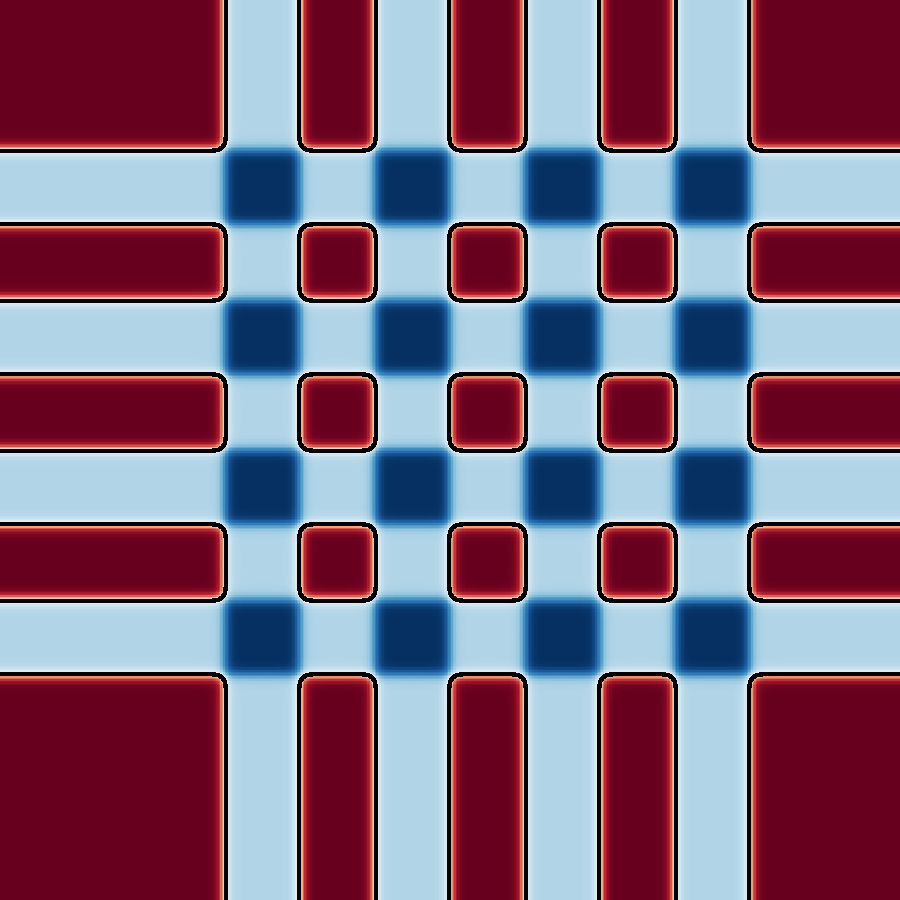
\includegraphics[width=0.4\textwidth]{figs/lower_bound_construction_clean.pdf}
  \caption{Visualization of the lower-bound construction in Proposition~\ref{prop:single-layer-lowerbound} for $n=2$, shown without the capping units: the function plotted is $\tfrac12+\delta+h_\lambda(x_1)+h_\lambda(x_2)$. The black lines indicate its zero set and the red regions are the regions where it is positive. The unbounded components visible towards the boundary of the picture are removed by the capping units.}
  \label{fig:lower-bound-construction}
\end{figure}

Finally, let $f(x)=f_\lambda(x/\lambda)$. Explicitly,
\[
f(x)=\tfrac12+\delta+\sum_{j=1}^n
\left[\sum_{k=1}^r(-1)^k\sigma(x_j-\lambda k)
-2\sigma(x_j-\lambda(r+1))-2\sigma(-x_j)\right].
\]
Its weights belong to $\{\pm e_1,\dots,\pm e_n\}$, so $q=L=1$. Its zero set is the image $\lambda\mathcal Z(f_\lambda)$, which preserves normal directions and Gauss-fibre cardinalities. Regularity and compactness are also preserved, proving~\eqref{eq:single-layer-lb}.
\end{proof}

\begin{remark}\label{rem:why-not-fewnomials}
The Bernstein bound uses the volume of the common support polytope. Real fewnomial estimates such as~\cite{bihansottile2007} instead depend on the number of monomials. These are different measures of complexity, so replacing Bernstein's theorem by a fewnomial bound does not automatically improve~\eqref{eq:single-layer-bound}.
\end{remark}

For greater depth, sigmoid composition prevents the direct Laurent-polynomial reduction. We formulate a fixed-depth extension as a conjecture.

\begin{conjecture}\label{conj:multi-layer-degree}
Fix $n,\ell,L\ge1$. Let $F:\R^n\to\R^m$ be a network with $\ell$ hidden layers of widths $n_1,\dots,n_\ell\ge n$, logistic sigmoid activations and affine outputs. Suppose the hidden-layer weight matrices have a common denominator $q\in\N_{>0}$, with all scaled entries bounded in absolute value by $L$. Then there is a constant $C(n,\ell,L)$ such that each pairwise difference with $0$ as a regular value satisfies
\begin{equation}\label{eq:multi-layer-bound}
\md\bigl(\mathcal Z(g_{ij})\bigr)
\le C(n,\ell,L)\left(\prod_{k=1}^\ell n_k\right)^n.
\end{equation}
Biases and affine-output coefficients may be arbitrary real numbers.
\end{conjecture}

Proposition~\ref{prop:single-layer-degree} proves the case $\ell=1$, with optimal width exponent by Proposition~\ref{prop:single-layer-lowerbound}. As a comparison, for fixed input dimension and depth, the number of linear regions of ReLU networks is bounded by $O_{n,\ell}(\prod_k n_k^n)$~\cite{raghu2017,serra2018,hanin2019}. ReLU networks lie outside the smooth Pfaffian setting; this comparison motivates the form of the conjecture but does not prove it.

The exponential growth in decision-region topology with depth established by Bianchini and Scarselli~\cite[Theorem~5 and Appendix~F]{bianchini2014complexity} is compatible with this conjecture, which concerns width dependence at fixed depth.

\subsection{Tubular neighbourhood bound for neural networks}\label{subsec:tube-nn}
A tube bound needs all section degrees $\md_i(V)$, not just $\md(V)$. An arbitrary affine section changes rational weight vectors into vectors with possibly irrational entries, so the preceding Laurent-polynomial argument does not directly give a uniform bound for sections. We instead retain the original coordinate exponentials as a global Pfaffian chain of length $n$.

\begin{proposition}\label{prop:single-layer-ideg}
Under the hypotheses of Proposition~\ref{prop:single-layer-degree}, put $D_0=2nLw$. For every $0\le i<n$,
\begin{equation}\label{eq:single-layer-ideg-precise}
\md_i(V)\le
2^{\frac{n(n-1)}2}D_0^{i+1}\bigl((i+1)D_0+1\bigr)^n.
\end{equation}
In particular,
\begin{equation}\label{eq:single-layer-ideg}
\md_i(V)\le K(n,L)w^{2n},\qquad
K(n,L):=2^{\frac{n(n-1)}2}(2nL)^n(2n^2L+1)^n.
\end{equation}
\end{proposition}

\begin{proof}
Use $G,D,y$ from~\eqref{eq:laurent-numerator}. Every exponent of $G$ lies in $[-Lw,Lw]^n$, so
\[
P(y)=(y_1\cdots y_n)^{Lw}G(y)
\]
is an ordinary polynomial of total degree at most $D_0$. The function
\[
\widetilde f(x)=P(y(x))=a(x)f(x),
\qquad
a(x)=(y_1(x)\cdots y_n(x))^{Lw}D(y(x))>0
\]
has the same regular zero set as $f$.

Parametrise a transverse affine section by $x=x_0+Ut$, where $t\in\R^d$, $d=i+1$, and $U\in\R^{n\times d}$ satisfies $U^{\trans}U=I_d$. The functions
\[
\eta_j(t)=\exp\!\left(-\frac{x_{0j}+(Ut)_j}{q}\right),\qquad 1\le j\le n,
\]
form a global autonomous chain on $\R^d$ of length $n$ and chain degree $1$, since
$\partial_{t_k}\eta_j=-(U_{jk}/q)\eta_j$. Put $\widehat f(t)=P(\eta_1(t),\dots,\eta_n(t))$. Both $\widehat f$ and its directional derivatives $\partial_\tau\widehat f$, for constant $\tau\in\R^d$, have degree at most $D_0$ in this chain. At each regular Gauss value, Lemma~\ref{le:gauss-nondegenerate} gives a non-degenerate system of $d$ such equations. Applying Theorem~\ref{thm:khovanskii} in $d$ variables gives
\[
2^{\frac{n(n-1)}2}D_0^d(dD_0-d+\min\{d,n\}+1)^n
=2^{\frac{n(n-1)}2}D_0^d(dD_0+1)^n.
\]
Taking suprema proves~\eqref{eq:single-layer-ideg-precise}. Since $1\le d\le n$ and $w,L\ge1$, this is at most the right-hand side of~\eqref{eq:single-layer-ideg}.
\end{proof}

The chain has length $n$ regardless of the width, and remains global even for irrational section directions. No logarithmic coordinates or constraints on the domain are needed.

\begin{theorem}\label{thm:prob_bound_single_layer}
Let $f,V$ satisfy Proposition~\ref{prop:single-layer-degree}, and let $X$ be uniform in any ball $B(p,\rho)$ with $\rho>0$. For every $\varepsilon>0$, writing $u=\varepsilon/\rho$,
\begin{equation}\label{eq:single-layer-prob-bound}
\prob\{\dist(X,V)\le\varepsilon\}
\le 2K(n,L)w^{2n}\bigl[(1+2u)^n-(1+u)^n\bigr].
\end{equation}
If in addition $V\subset B(p,\rho)$, the bracket can be replaced by $(1+u)^n-1$.
\end{theorem}

\begin{proof}
Substitute~\eqref{eq:single-layer-ideg} into Proposition~\ref{prop:local-tube} and use
\[
\sum_{i=0}^{n-1}\binom n{i+1}u^{i+1}(1+u)^{n-i-1}
=(1+2u)^n-(1+u)^n.
\]
If $V\subset B(p,\rho)$, apply Theorem~\ref{thm:tube_bound} directly to $V$ and divide by $\omega_n\rho^n$.
\end{proof}

A one-variable zero count improves the leading coefficient.

\begin{lemma}\label{lem:polya}
A nonzero exponential polynomial $E(t)=\sum_{j=1}^M d_j\econst^{\nu_jt}$ with distinct real frequencies has at most $M-1$ distinct real zeros.
\end{lemma}

\begin{proof}
Discard zero coefficients and argue by induction on $M$. Multiplication by $\econst^{-\nu_1t}$ preserves zeros, and differentiation leaves an exponential polynomial with $M-1$ frequencies. Rolle's theorem bounds the zeros of the original function by one more than those of its derivative.
\end{proof}

\begin{lemma}\label{lem:line-intersection}
For $f$ as in Proposition~\ref{prop:single-layer-degree}, its restriction to any affine line has at most $(2Lw+1)^n-1$ isolated real zeros.
\end{lemma}

\begin{proof}
On a line $x=x_0+tv$, multiply $f(x)$ by the positive denominator $D(y(x))$. Expanding~\eqref{eq:laurent-numerator} gives an exponential polynomial whose frequencies are
\[
-\frac1q\left\langle\sum_{k=1}^w \kappa_kp_k,v\right\rangle,
\qquad \kappa\in\{0,1\}^w.
\]
The integer vectors $\sum_k\kappa_kp_k$ lie in $[-Lw,Lw]^n$, so there are at most $(2Lw+1)^n$ distinct frequencies. If the resulting polynomial is nonzero, apply Lemma~\ref{lem:polya}; if it is identically zero, the restriction has no isolated zeros.
\end{proof}

\begin{corollary}\label{cor:single-layer-tight-prob-bound}
Under the hypotheses of Theorem~\ref{thm:prob_bound_single_layer}, let $a_w=(2Lw+1)^n-1$. Then
\begin{align}
\prob\{\dist(X,V)\le\varepsilon\}\le{}&
2na_wu(1+u)^{n-1}\nonumber\\
&+2K(n,L)w^{2n}
\bigl[(1+2u)^n-(1+u)^n-nu(1+u)^{n-1}\bigr].
\label{eq:single-layer-refined-tube}
\end{align}
In particular, for all $u>0$,
\begin{equation}\label{eq:single-layer-linear-tube}
\prob\{\dist(X,V)\le\varepsilon\}
\le\min\{1,H(n,L)w^nu\},
\end{equation}
where one may take
\begin{equation}\label{eq:single-layer-H}
H(n,L)=2^nn(2L+1)^n+
2K(n,L)\bigl(3^n-2^n-n2^{n-1}\bigr).
\end{equation}
\end{corollary}

\begin{proof}
Transverse line sections consist of isolated zeros, so Lemma~\ref{lem:line-intersection} gives $\md_0(V)\le a_w$. Use this for the $i=0$ term of~\eqref{eq:local-tube}, and~\eqref{eq:single-layer-ideg} for the remaining terms, to obtain~\eqref{eq:single-layer-refined-tube}.

Put $z=w^nu$. If $z\le1$, then $u\le1$ and the first term is at most $2^nn(2L+1)^nz$. For the remaining terms, $u^{i+1}\le u^2$ and $(1+u)^{n-i-1}\le2^{n-i-1}$ for $i\ge1$. Thus their sum is at most
\[
2K(n,L)z^2
\sum_{i=1}^{n-1}\binom n{i+1}2^{n-i-1}
=2K(n,L)z^2(3^n-2^n-n2^{n-1}).
\]
Use $z^2\le z$. If $z>1$, the trivial probability bound suffices since $H(n,L)\ge1$. This proves~\eqref{eq:single-layer-linear-tube}.
\end{proof}

For $u\to0$, the refined bound has expansion $2na_wu+O_{n,L}(w^{2n}u^2)$, with the remainder uniform for $w\ge1$ and $0\le u\le1$. The width exponent in this probability bound is an upper estimate; Proposition~\ref{prop:single-layer-lowerbound} establishes sharpness only for the Gauss-map degree.

The regular-value hypothesis can be removed from the linear-radius estimate by approximating the zero set from both signs using an elementary hypersurface approximation principle; compare the discussion of nearby levels in the introduction of~\cite{basu2021hausdorff}. Using two levels of $f$ preserves the shallow network architecture.

\begin{corollary}\label{cor:single-layer-singular-linear}
Let $f$ have the representation and weight assumptions of Proposition~\ref{prop:single-layer-degree}, but replace its regular-value hypothesis by $f\neq0$. Put $V=\mathcal Z(f)$, and let $X$ be uniform in $B(p,\rho)$, where $\rho>0$. Then, for every $\varepsilon>0$,
\[
\prob\{\dist(X,V)\le\varepsilon\}
\le\min\left\{1,2H(n,L)w^n\frac{\varepsilon}{\rho}\right\},
\]
where $H(n,L)$ is given by~\eqref{eq:single-layer-H}.
\end{corollary}

\begin{proof}
If $V$ is empty, the assertion is immediate. Otherwise $f$ is nonconstant. By Sard's theorem, choose $\delta_j\rightarrow 0$ such that both $\delta_j$ and $-\delta_j$ are regular values of $f$, and set
\[
V_j^+=\{f=\delta_j\},\qquad
V_j^-=\{f=-\delta_j\},\qquad A_j=V_j^+\cup V_j^-.
\]
Each nonempty $V_j^\pm$ is a regular zero set of a shallow network with the same $n,w,L$ as $f$: only the affine-output bias changes. Consequently, Corollary~\ref{cor:single-layer-tight-prob-bound} and the union bound give, for every $r>0$,
\begin{equation}\label{eq:two-level-tube}
\prob\{\dist(X,A_j)\le r\}
\le\min\{1,2H(n,L)w^n r/\rho\}.
\end{equation}

For every $z\in V$, we have $\dist(z,A_j)\to0$. Indeed, analyticity and $f\not\equiv0$ imply that every neighbourhood of $z$ contains a point $y$ with $f(y)\ne0$. For all sufficiently large $j$, the intermediate value theorem along the segment from $z$ to $y$ gives a point of $A_j$ on that segment. Taking $y$ arbitrarily close to $z$ proves the claim. Both signs are needed because $f$ may have a local maximum or minimum at a zero.

Since $V$ is nonempty and closed, a nearest point in $V$ exists for every $x\in\R^n$. The preceding claim therefore implies
\[
\limsup_{j\to\infty}\dist(x,A_j)\le\dist(x,V).
\]
For every $\eta>0$, it follows that
\[
\mathbf1_{\{\dist(x,V)\le\varepsilon\}}
\le\liminf_{j\to\infty}
\mathbf1_{\{\dist(x,A_j)\le\varepsilon+\eta\}}.
\]
Apply Fatou's lemma under the uniform probability measure, use~\eqref{eq:two-level-tube} with $r=\varepsilon+\eta$, and let $\eta$ go to zero.
\end{proof}

\begin{remark}
This estimates the full distance neighbourhood, including near singular points. If $V$ has real codimension $c>1$, it still gives only linear decay in $\varepsilon/\rho$; it does not give the sharper $(\varepsilon/\rho)^c$ behaviour sought in dimension-sensitive tube bounds. The exclusion $f\equiv0$ is essential, since then $V=\R^n$ and the probability is one at every radius.
\end{remark}
